\documentclass[12pt, psamsfonts]{amsart}

%-------Packages---------
\usepackage{amssymb,amsfonts}
\usepackage{fullpage}
\usepackage{todonotes}
\usepackage{physics}
\usepackage[all,arc]{xy}
\usepackage{enumerate}
\usepackage{mathrsfs}
\usepackage{theoremref}
\usepackage{graphicx}
\usepackage[bookmarks]{hyperref}

%--------Theorem Environments--------
%theoremstyle{plain} --- default
\newtheorem{thm}{Theorem}[section]
\newtheorem{cor}[thm]{Corollary}
\newtheorem{prop}[thm]{Proposition}
\newtheorem{lem}[thm]{Lemma}
\newtheorem{conj}[thm]{Conjecture}
\newtheorem{quest}[thm]{Question}

\theoremstyle{definition}
\newtheorem{defn}[thm]{Definition}
\newtheorem{defns}[thm]{Definitions}
\newtheorem{con}[thm]{Construction}
\newtheorem{exmp}[thm]{Example}
\newtheorem{exmps}[thm]{Examples}
\newtheorem{notn}[thm]{Notation}
\newtheorem{notns}[thm]{Notations}
\newtheorem{addm}[thm]{Addendum}
\newtheorem*{exer}{Exercise}

\theoremstyle{remark}
\newtheorem{rem}[thm]{Remark}
\newtheorem{rems}[thm]{Remarks}
\newtheorem{warn}[thm]{Warning}
\newtheorem{sch}[thm]{Scholium}

\DeclareMathOperator{\Hom}{Hom}
\DeclareMathOperator{\Id}{Id}

\makeatletter
\let\c@equation\c@thm
\makeatother
\numberwithin{equation}{section}

\bibliographystyle{plain}

\begin{document}

\title{Math 611 Homework (Due 9/18)}
\author{Hidenori Shinohara}
\maketitle


\begin{exer}{(Problem 12, Chapter 1.2)}
  The Klein bottle is usually pictured as a subspace of $\mathbb{R}^3$ like the subspace $X \subset \mathbb{R}^3$ shown in the first figure at the right.
  If one wanted a model that could actually function as a bottle, one would delete the open disk bounded by the circle of self-intersection of $X$, producing a subspace $Y \subset X$.
  Show that $\pi_1(X) \approx \mathbb{Z} * \mathbb{Z}$ and that $\pi_1(Y)$ has the presentation $\langle a, b, c \mid aba^{-1}b^{-1}cb^{\epsilon}c^{-1} \rangle$ for $\epsilon = \pm 1$.
  Show also that $\pi_1(Y)$ is isomorphic to $\pi_1(\mathbb{R}^3 \setminus Z)$ for $Z$ the graph shown in the figure.
\end{exer}

\begin{proof}
  We will construct $X$ from the 1-skeleton in Figure \ref{fig:fund_x_klein}.
  \begin{figure}
    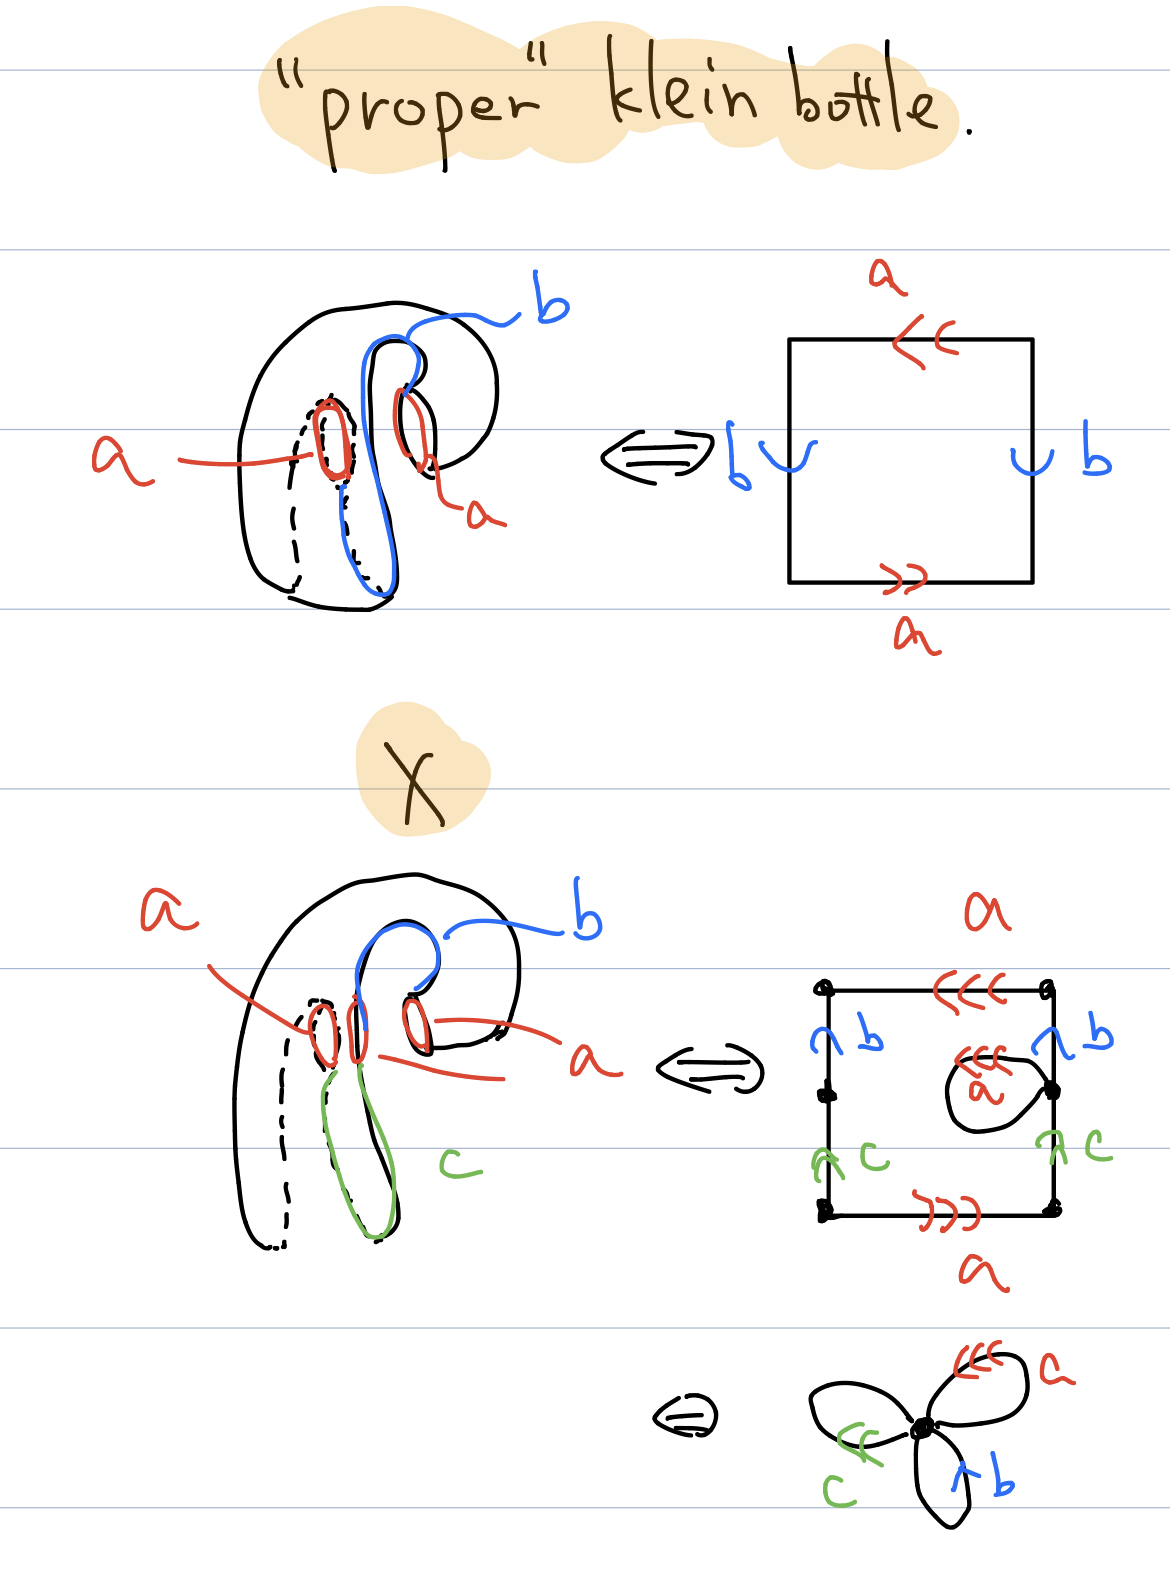
\includegraphics[width=.5\linewidth]{klein_solution_zz.jpeg}
      \caption{Fundamental Group of $X$}
    \label{fig:fund_x_klein}
  \end{figure}
  The 1-skeleton has three loops $a, b, c$, so the fundamental group is $\langle a, b, c \mid \rangle$.
  The main difference between $X$ and the ``proper" Klein bottle is that the loop $a$ actually gets glued on the surface.
  Thus we will glue the first 2-cell to $a$, and another 2-cell on the loop $c^{-1}acbab^{-1}$.
  Therefore, we end up with the fundamental group $\langle a, b, c \mid a, c^{-1}aca^{-1}bab^{-1} \rangle$.
  Then $\langle a, b, c \mid a, c^{-1}acabab^{-1} \rangle \approx \langle b, c \mid \rangle \approx \mathbb{Z} * \mathbb{Z}$ since the relation $c^{-1}aca^{-1}bab^{-1}$ is trivial by the relation $a$.

  In order to calculate the fundamental group of $Y$, it suffices to repeat the following step without attaching a 2-cell to $a$.
  Thus the fundamental group is $G = \langle a, b, c \mid c^{-1}aca^{-1}bab^{-1} \rangle$.
  This is isomorphic to the group given in the textbook, $H = \langle a, b, c \mid aba^{-1}b^{-1}cbc^{-1} \rangle$ by $\phi: G \rightarrow H$ that maps $a$ to $b$, $b$ to $c$, and $c$ to $a^{-1}$.
\end{proof}

\begin{exer}{(Problem 14, Chapter 1.2)}
  Consider the quotient space of a cube $I^3$ obtained by identifying each square face with the opposite square face via the right-handed screw motion consisting of a translation by one unit in the direction perpendicular to the face combined with a one-quarter twist of the face about its center point.
  Show this quotient space $X$ is a cell complex with two 0-cells, four 1-cells, three 2-cells, and one 3-cell.
  Using this structure, show that $\pi_1(X)$ is the quaternion group $\{ \pm 1, \pm i, \pm j, \pm k \}$ of order eight.
\end{exer}

\begin{proof}
  \begin{figure}
    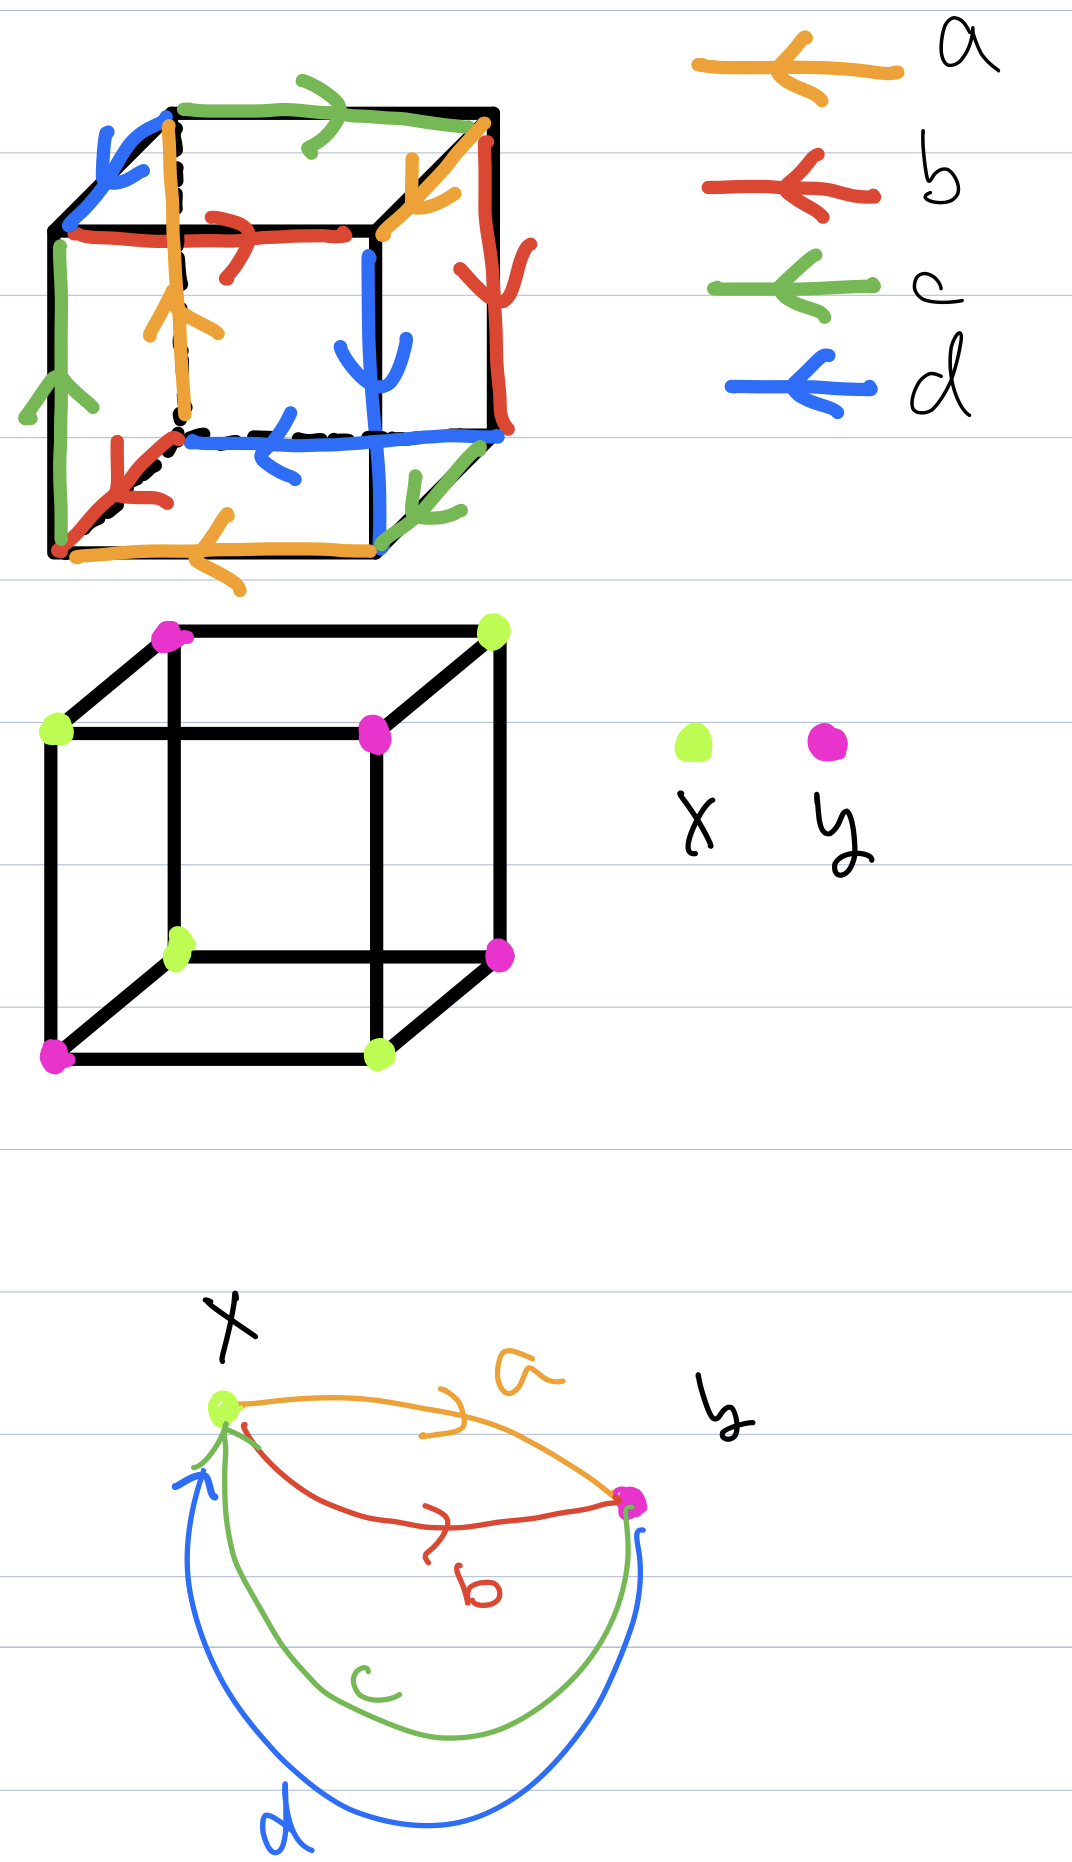
\includegraphics[width=.5\linewidth]{cube.jpeg}
    \caption{Problem 14}
    \label{fig:cube}
  \end{figure}
  The vertices and edges get identified as in Figure \ref{fig:cube}.
  Thus we have two 0-cells and four 1-cells.
  Since the opposite faces are identified and the cube has 6 faces, we need to glue three 2-cells to the cube.
  Lastly, we need a 3-cell glued to the three faces.
  By Proposition 1.26, the fundamental group of a 2-skeleton is the same as the fundamental group of a space obtained by attaching 3-cells, so it suffices to consider the fundamental group we obtain by attaching the three 2-cells to the graph.
  As in Figure \ref{fig:cube}, the graph has 4 edges between two vertices.
  The fundamental group of this is $\langle ab^{-1}, ac, ad \rangle$ because by ``shrinking" $a$ we obtain the graph consisting of one vertex and three loops.
  By attaching a 2-cell to each of the top-bottom pair, left-right pair, and the front-back pair, we obtain

  \begin{align*}
    \langle ac, ab^{-1}, ad \mid ab^{-1}d^{-1}c, adc^{-1}b^{-1}, acbd \rangle.
  \end{align*}

  Thus this is the fundamental group of the given space.
  We claim that $(ac)^2 = (ab^{-1})^2 = (ad)^2 = (ac)(ab^{-1})(ad)$.

  \begin{itemize}
    \item
      $(ac)^2 = (ab^{-1})^2$?
      \begin{align*}
        ac = d^{-1}b^{-1}
          &\implies ab^{-1}bc = d^{-1}b^{-1} \\
          &\implies ab^{-1}ad = d^{-1}b^{-1} \\
          &\implies ab^{-1}a = d^{-1}b^{-1}d^{-1} \\
          &\implies ab^{-1}ab^{-1} = d^{-1}b^{-1}d^{-1}b^{-1} \\
          &\implies (ab^{-1})^2 = (d^{-1}b^{-1})^2 \\
          &\implies (ab^{-1})^2 = (ac)^2.
      \end{align*}
    \item
      $(ac)^2 = (ad)^2$?
      \begin{align*}
        ab^{-1} = c^{-1}d
          &\implies cab^{-1} = d \\
          &\implies ca = db \\
          &\implies cac = dbc \\
          &\implies cac = dad \\
          &\implies acac = adad \\
          &\implies (ac)^2 = (ad)^2.
      \end{align*}
    \item
      $(ad)^2 = (ac)(ab^{-1})(ad)$?
      $(ac)(ab^{-1}) = acc^{-1}d = ad$, so $(ac)(ab^{-1})(ad) = (ad)^2$.
  \end{itemize}

  Moreover, we claim that $(ac)^2 \ne e$ and $(ac)^4 = e$.

  \begin{itemize}
    \item
      $(ac)^2 \ne e$.
      \todo[inline]{
        Prove this!
      }
    \item
      $(ac)^4 = e$.
      \todo[inline]{
        Prove this!
      }
  \end{itemize}
  
\end{proof}

\begin{exer}{(Problem 22, Chapter 1.2)}
  $ $
  \begin{itemize}
    \item
      Show that $\pi_1(\mathbb{R}^3 - K)$ has a presentation with one generator $x_i$ for each strip $R_i$ and one relation of the form $x_ix_jx_i^{-1} = x_k$ for each square $S_l$,
      where the indices are as in the figures above.
  \end{itemize}
\end{exer}

\begin{proof}
  $ $
  \begin{itemize}
    \item
      We will construct the 2-dimensional complex $X$ by first attaching $R_i$'s.
      We will attach $R_i$ one by one.
      We begin with a plane $\mathbb{R}^2$ whose fundamental group is $0$.
      A rectangular strip $R_i$ has a fundamental group isomorphic to $\mathbb{Z}$ since it is homotopy equivalent to $S^1$.
      Thus it is a free group with one generator.
      We will calculate the fundamental group of a space we obtain after attaching $T$ to $R_i$ using Van Kampen.
      The intersection is a rectangle, so the intersection is simply connected.
      Thus the fundamental group of the new space is simply the free product of $T$ and $R_i$.
      Therefore, the fundamental group of the space we obtain by attaching all the $R_i$'s is $\langle x_1, \cdots, x_n \mid \rangle$ where $n$ is the number of $R_i$'s and each $x_i$ corresponds to $R_i$.

      Now, we will attach $S_l$'s and we will do so one by one.
      The fundamental group of each $S_l$ is $0$ since each $S_l$ is simply connected.
      Thus attaching $S_l$'s does not add any new generators to the fundamental group.
      \begin{figure}
        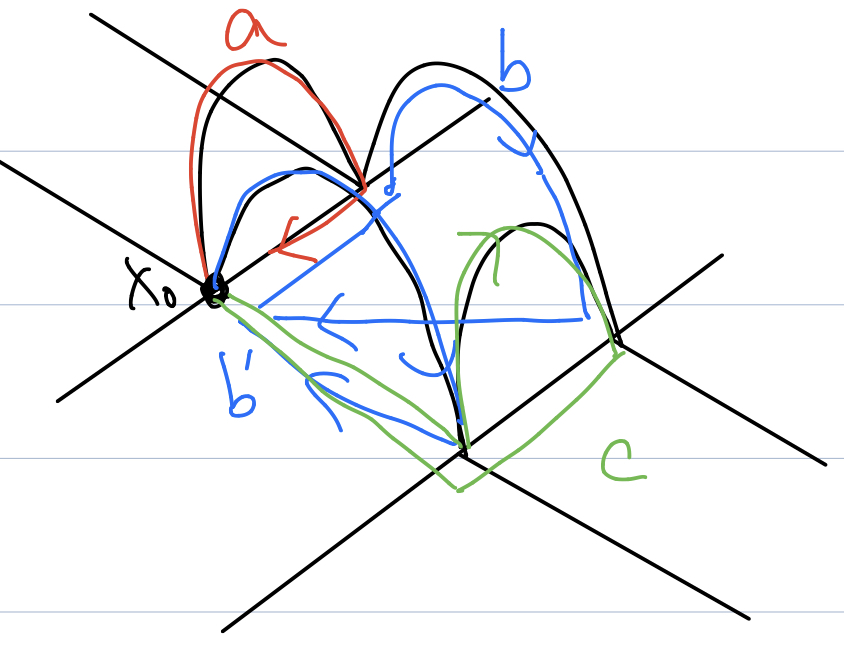
\includegraphics[width=.5\linewidth]{wirtinger.jpeg}
        \caption{Wirtinger presentation}
        \label{fig:wirtinger}
      \end{figure}
      Figure \ref{fig:wirtinger} shows the intersection between an $S_l$ and the current space $X$.
      $a, b, b', c$ denote loops based at $x_0$, and $[b] = [b']$.
      Moreover, $[a], [b], [c]$ are exactly the generator of the corresponding rectangular strip.
      We will consider the intersection between $S_l$ and $X$.
      \begin{itemize}
        \item
          The loop that goes through the intersection is path homotopic to $abc^{-1}b^{-1}$ in $X$.
        \item
          The loop that goes through the intersection is nulhomotopic in $S_l$ since $S_l$ is simply connected.
      \end{itemize}
      By Van Kampen, the new group is $\pi_1(X) * \pi_1(S_l) / (i_{X}(g)i_{S_l}(g)^{-1})$ where $g$ is any loop in the intersection.
      Since $\pi_1(S_l) = 0$, $i_{S_l}(g) = e$ for any $g$.
      Then $(i_X(g)) = ([abc^{-1}b^{-1}])$ since the intersection is homeomorphic to $S^1$ and $[abc^{-1}b^{-1}]$ is a generator.
      Since $\pi_1(S_l) = 0$, we have $\pi_1(X) / ([a][b][c^{-1}][b^{-1}])$.

      After attaching all the $S_l$'s we will end up with $\langle x_1, \cdots, x_n \mid [a_l][b_l][c_l^{-1}][b_l^{-1}] \rangle$ where

      \begin{itemize}
        \item
          For each $S_l$, we add a relation $[a_l][b_l][c_l^{-1}][b_l^{-1}]$.
          Note that this means $[a_l][b_l][c_l^{-1}][b_l^{-1}] = e$, so $[a_l] = [b_l][c_l][b_l^{-1}]$, and this is exactly the desired relation.
        \item
          Each $x_i$ corresponds to a rectangular strip $R_i$.
          These are the only generators because $S_l$'s are all simply connected.
      \end{itemize}
    \item
      The abelianization of $\pi_1(\mathbb{R}^3 - K)$ turns a relation $x_ix_jx_i^{-1} = x_k$ into $x_j = x_k$.
      In other words, this implies that, at each square $S_l$, the generators for the two strips that are ``separated" by the middle strip are identified.
      Let $x_i, x_j$ be two distinct generators.
      Since $K$ is a knot, there exists a finite sequence $x_i = x_{i_0}, \cdots, x_{i_k} = x_j$ of generators such that the corresponding strips $R_{i_0}, \cdots, R_{i_k}$ are next to each other.
      (See Figure \ref{fig:separated_knots})
      \begin{figure}
        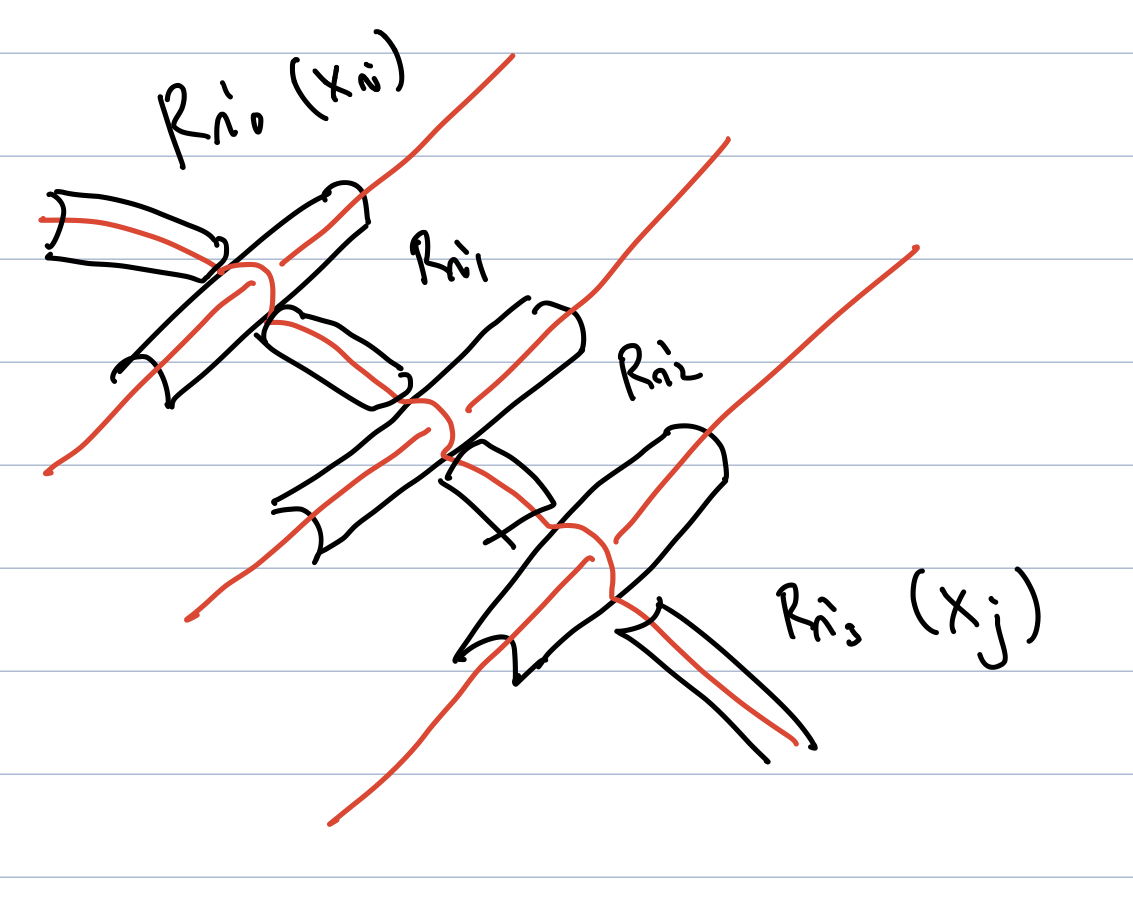
\includegraphics[width=.5\linewidth]{separated_knots.jpeg}
        \caption{Problem 22 (b)}
        \label{fig:separated_knots}
      \end{figure}
      Since each intersection has a square, $x_{i_t} = x_{i_{t + 1}}$ for each $t$.
      (For instance, in Figure \ref{fig:separated_knots}, $x_{i_0} = x_{i_1}$ because of the intersection between $R_{i_0}$ and $R_{i_1}$. Similarly, $x_{i_1} = x_{i_2}$ and $x_{i_2} = x_{i_3}$.)
      Therefore, $x_i = x_{i_0} = x_{i_1} = \cdots = x_{i_k} = x_j$.

      This implies that any two generators are identified after the abelianization.
      Hence, $\pi_1(\mathbb{R}^3 - K)$ is a free group with one generator and no relations, so it is isomorphic to $(\mathbb{Z}, +)$.
  \end{itemize}

\end{proof}

\end{document}


